\documentclass[../main.tex]{subfiles}

\begin{document}
\section{CHIPs Architecture}
The CHIPS architecture is an amalgamation of chiplets connected through an interposer. This structure is known as two and a half Dimensions (2.5D), and this structure is the foundation of the CHIPS architecture. The technology that allows chiplets to communication through an interposer is (AIB) advanced interface bus\cite{AIBWhitePaper}. This bus severs as the physical layer in the protocol stack. All chiplets use AXI as the next layer in the protocol stack. AXI is the protocol that makes up the buck of the SOC for the CHIPS architecture.

\subsection{2.5D Structure}
All chiplets share a standard interface in the CHIPS architecture, AIB interface. This interface allows chiplet to chiplet communication through an interposer, and figure \ref{fig:AIBInterposer} shows the structure of this interface. Each chiplet's IO consists of an AIB driver. This driver is capable of running at a single data rate (SDR) or double data rate (DDR). SDR is the configuration used in the CHIPS architecture. The AIB drivers work in pairs, one set to transmit and the other set to receive. Figure \ref{fig:AIBInterface} shows a standard configuration of drivers. An AIB channel is a collection of AIB drivers, and figure \ref{fig:AIBChannel} shows one such channel.  For transfer data across this interface, one channel must be a master, and the other must be a slave. The AIB interface makes up the lowest link in the protocol stack. The next physical link in the protocol stack is the AXI interface, and all the chiplets share this interface.    

\begin{figure}
    \centering
    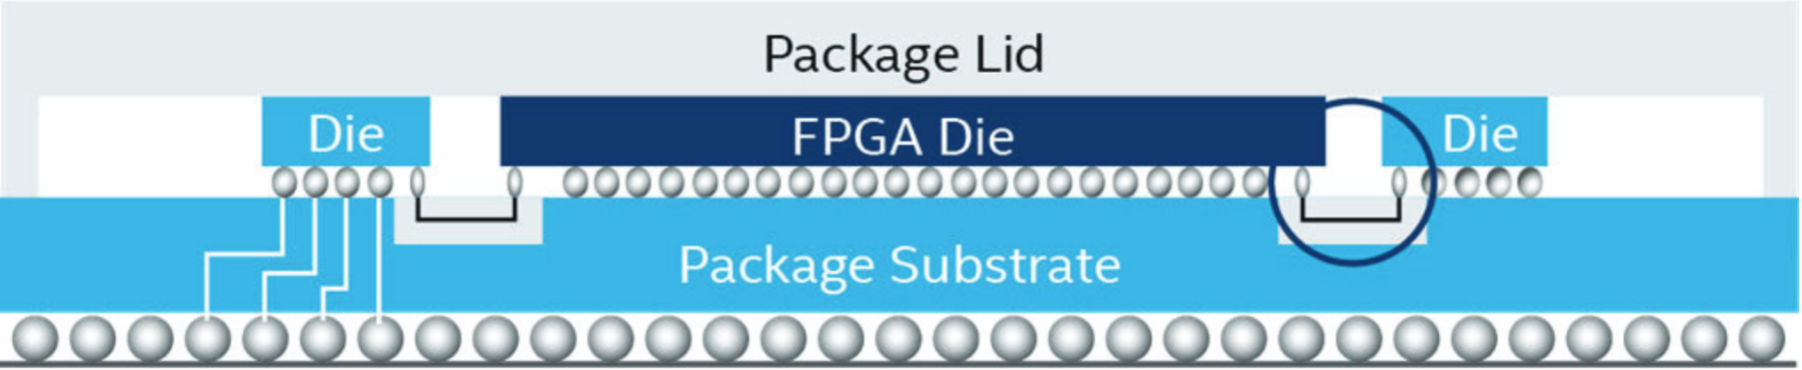
\includegraphics[scale=.25]{pngs/Interposer.png}
    \caption{AIB Interposer Connection\cite{AIBWhitePaper}}
    \label{fig:AIBInterposer}
\end{figure}
\begin{figure}
    \centering
    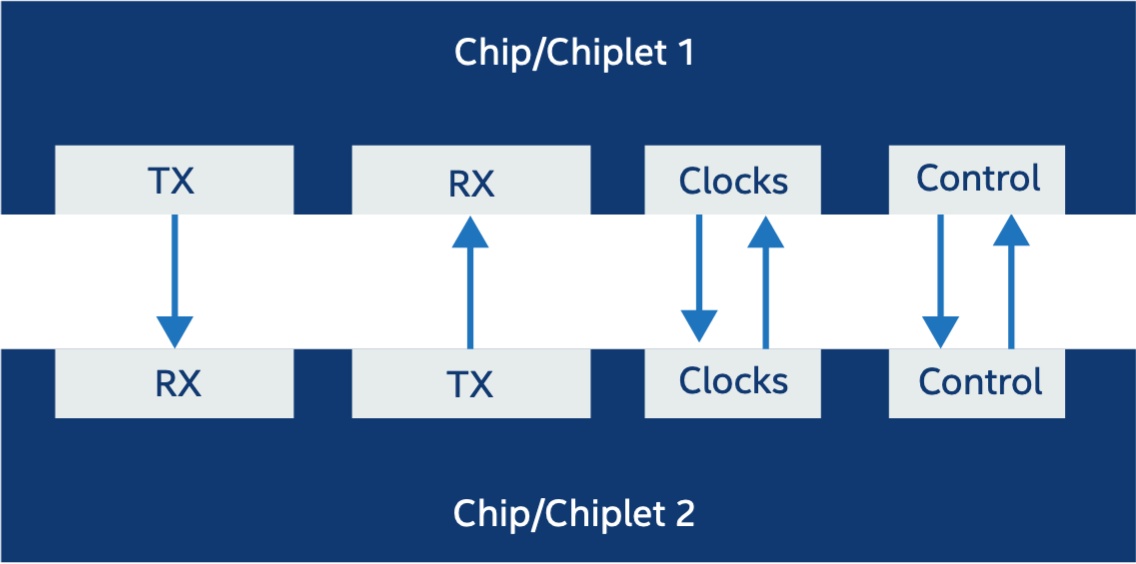
\includegraphics[scale=.4]{pngs/AIB-interface.png}
    \caption{AIB Interface\cite{AIBWhitePaper}}
    \label{fig:AIBInterface}
\end{figure}

\begin{figure}
    \centering
    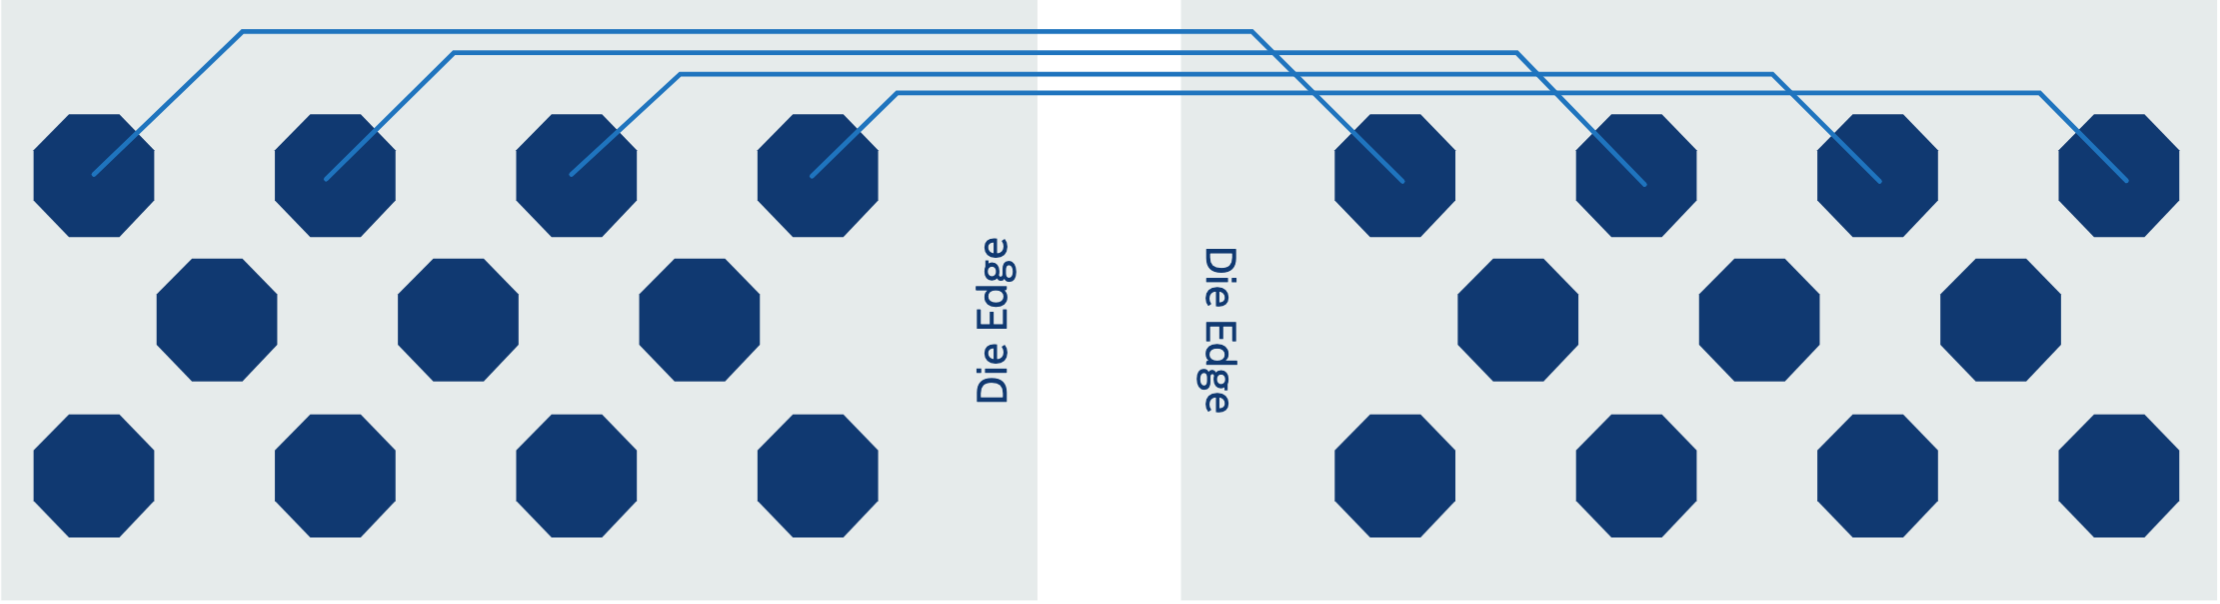
\includegraphics[scale=.2]{pngs/AIB-Channel.png}
    \caption{AIB Channel Connection\cite{AIBWhitePaper}}
    \label{fig:AIBChannel}
\end{figure}

An AIB channel in the CHIPS architecture is made up of 48 drivers. The drivers are broken up into two functions: one is data transfer, and the other is transmitting or receiving 4 sets of differential clocks. The lower 40 drivers are for data, and the upper 8 are for clocks. The configuration of the drivers depends on which side of the AIB interface the driver is on. For master, the data drivers are set to transmit, and the other drivers are set to receive, and the same goes for the clocks. Theses clocks create an async boundary around each chiplet. 

\begin{figure}
    \centering
    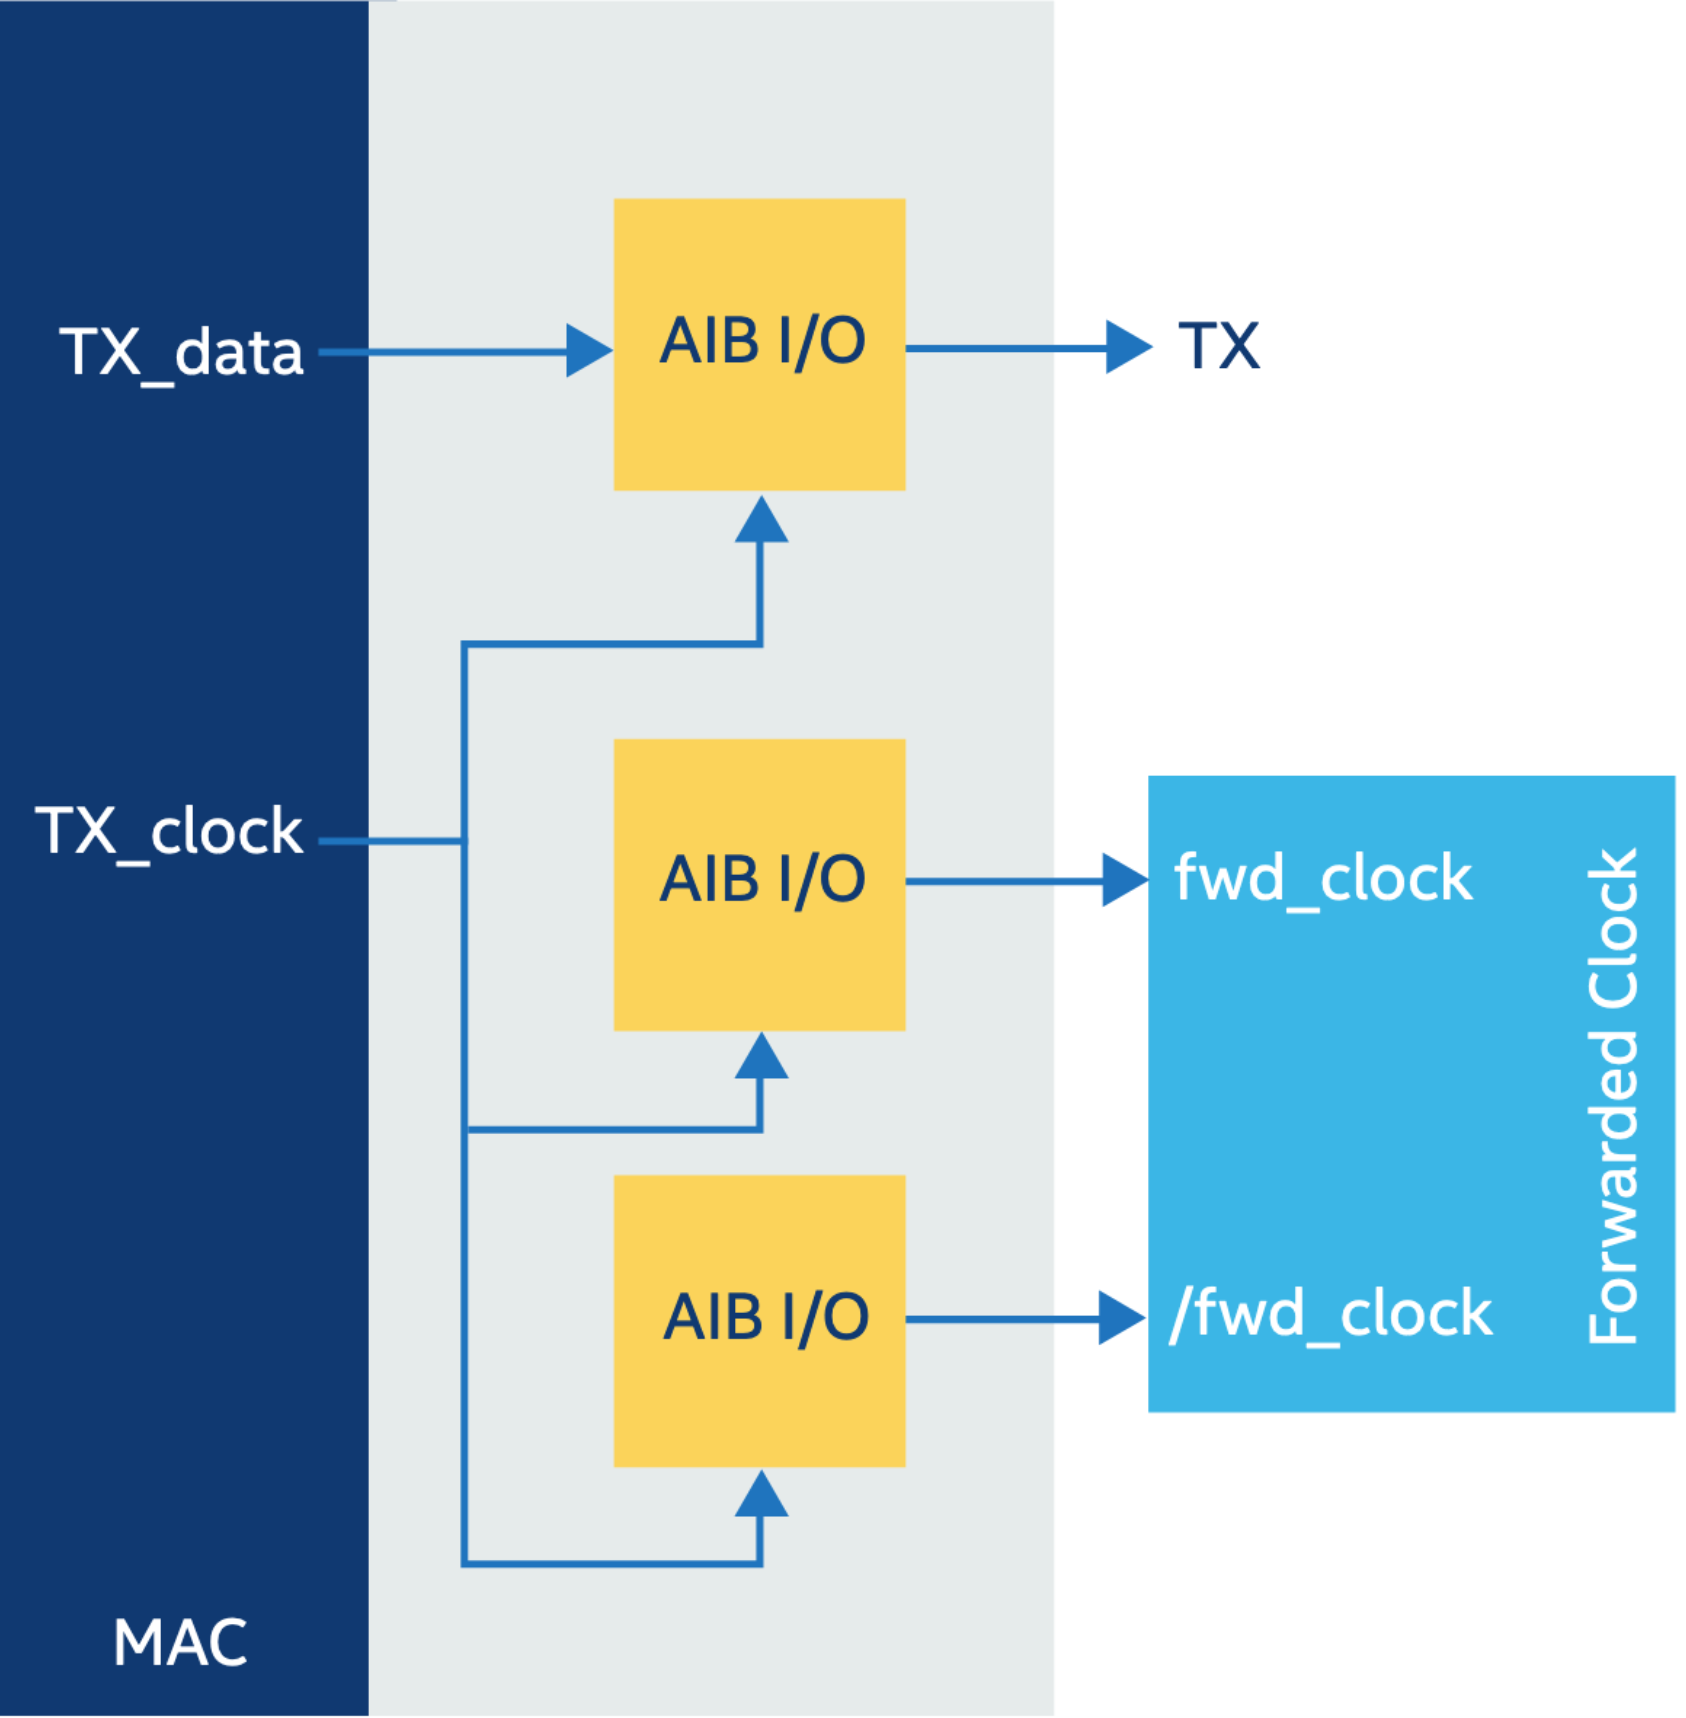
\includegraphics[scale=.2]{pngs/AIB-Tx.png}
    \caption{Transmitting\cite{AIBWhitePaper}}
    \label{fig:AIB-Tx}
\end{figure}

\begin{figure}
    \centering
    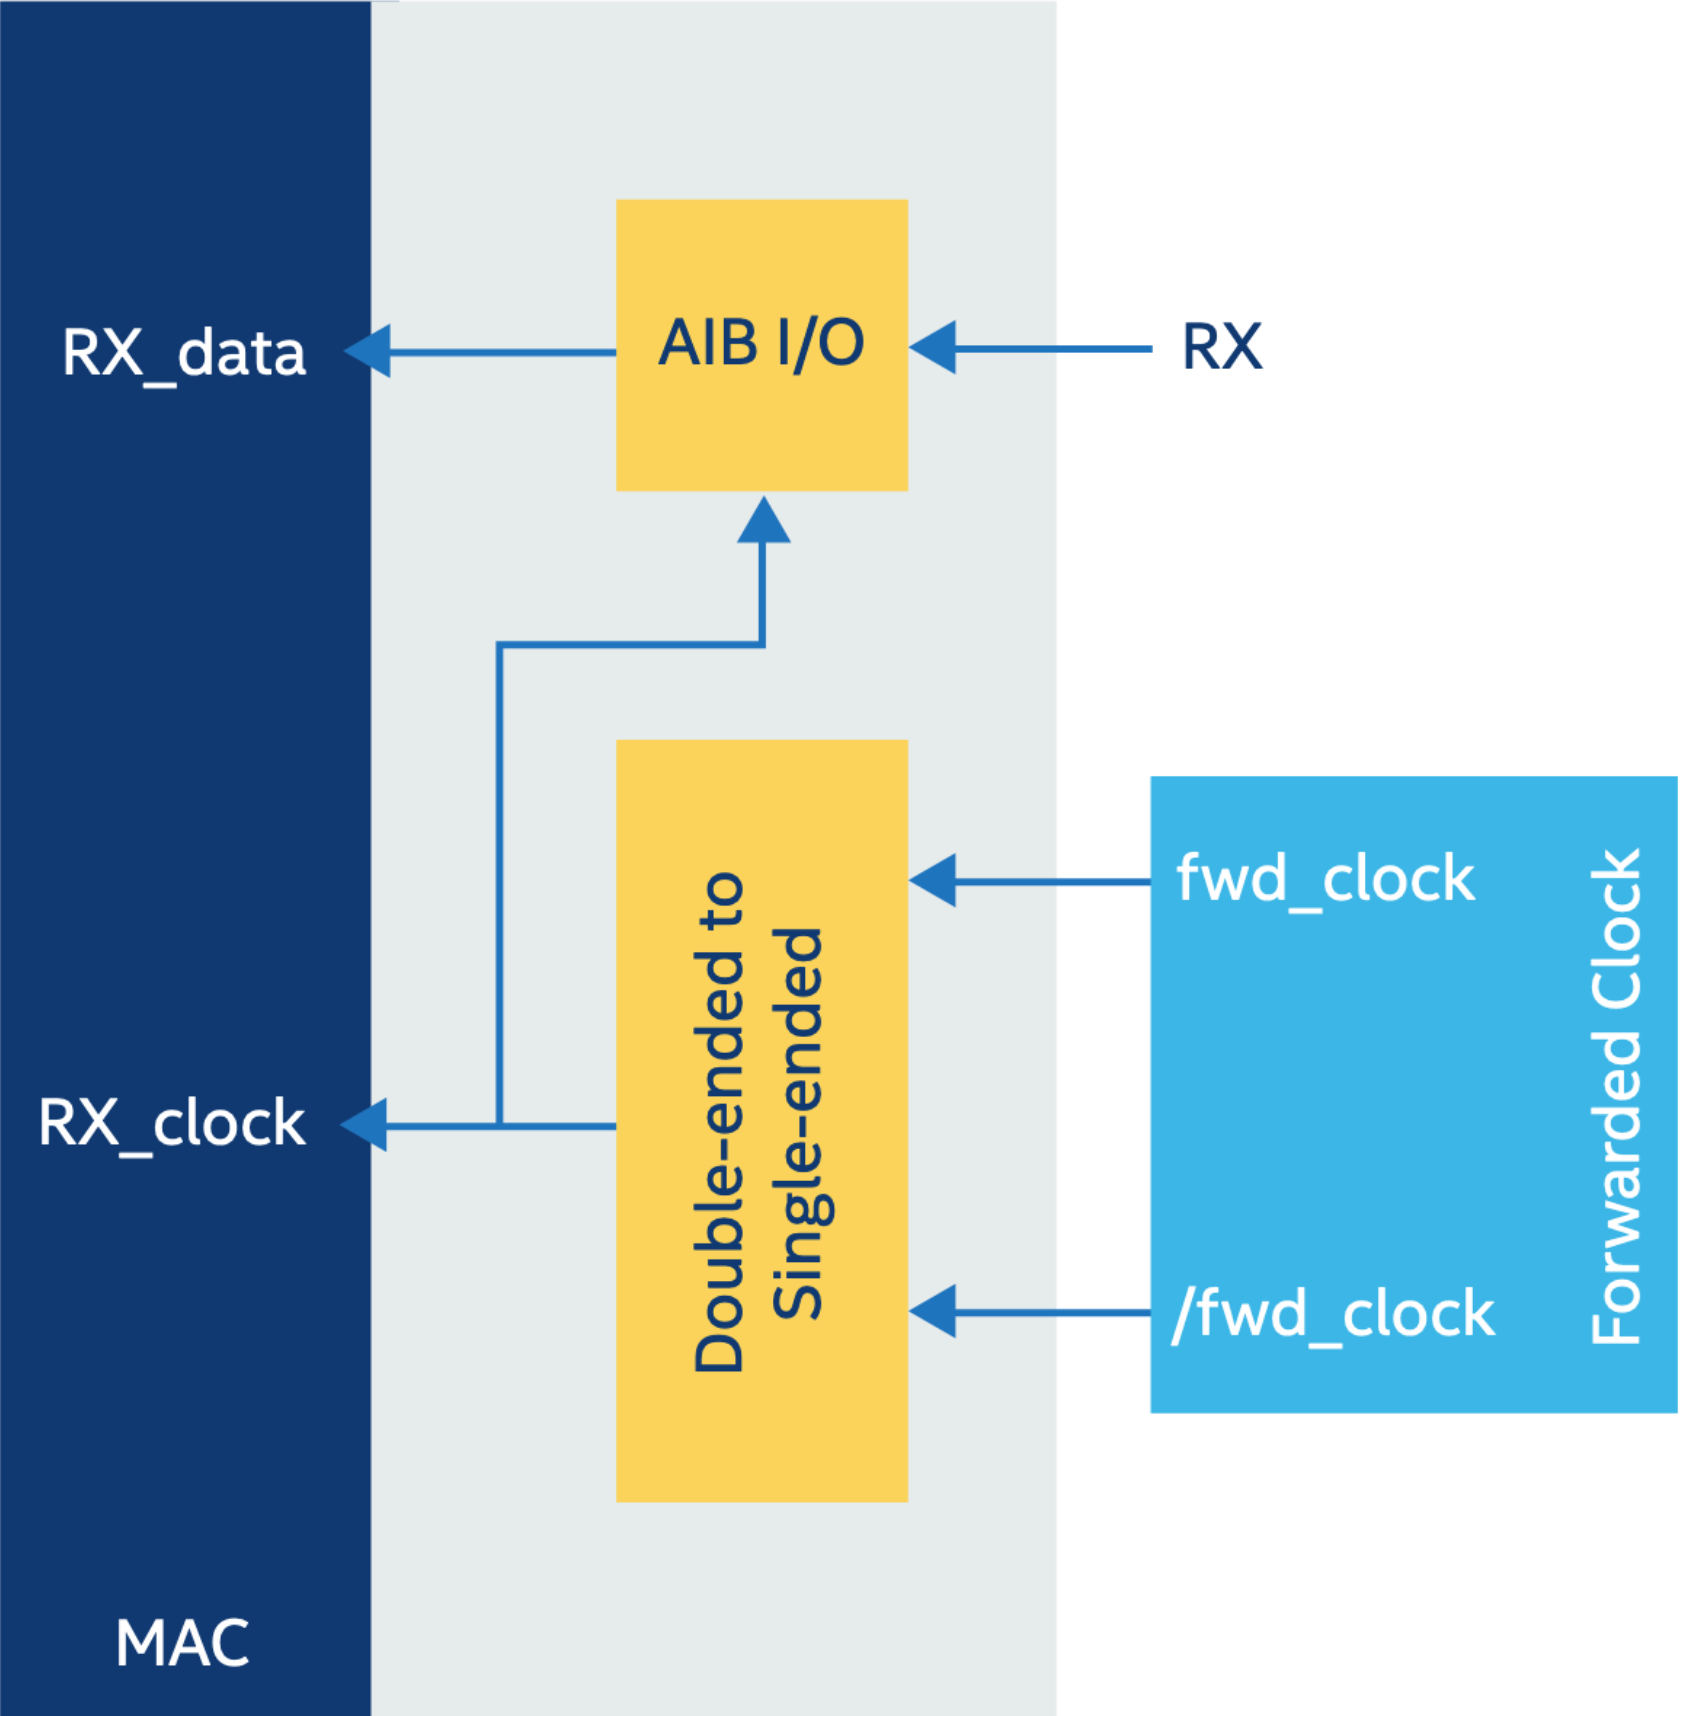
\includegraphics[scale=.2]{pngs/AIB-Rx.png}
    \caption{Receiving\cite{AIBWhitePaper}}
    \label{fig:AIB-Rx}
\end{figure}

\begin{figure}
    \centering
    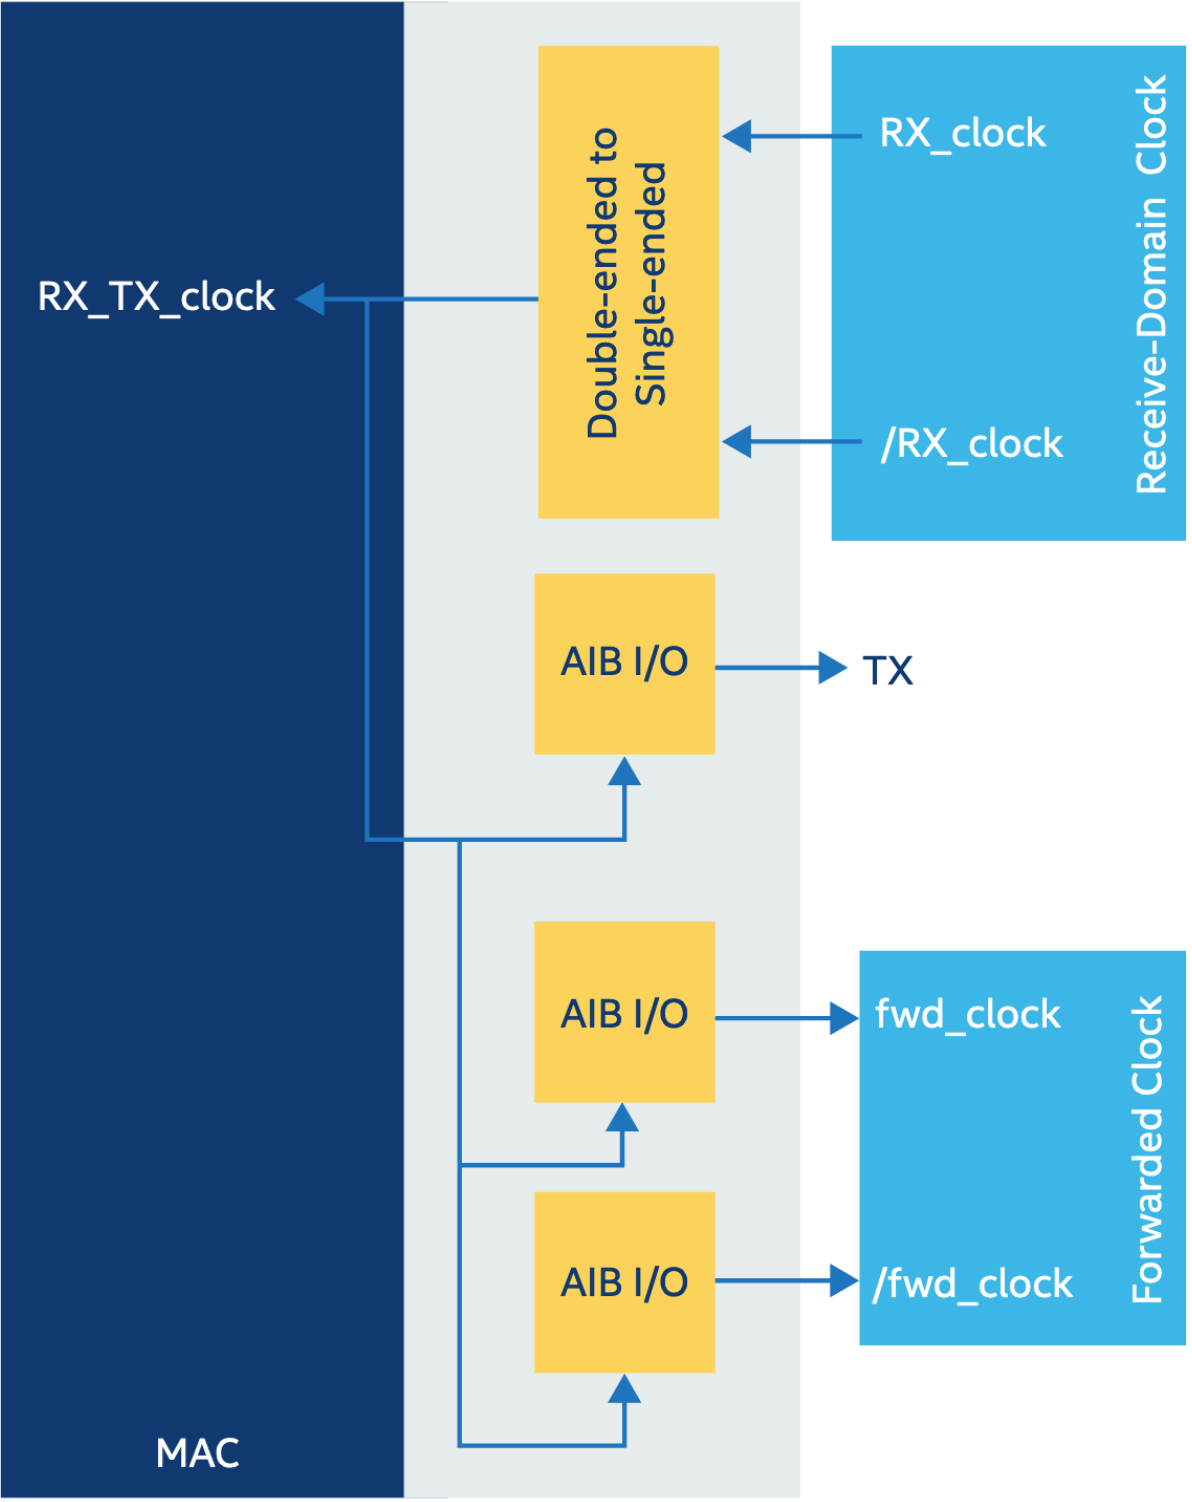
\includegraphics[scale=.27]{pngs/AIB-Rx-Tx.png}
    \caption{Forwarding\cite{AIBWhitePaper}}
    \label{fig:AIB-Rx-Tx}
\end{figure}


The four clocks are broken up into two groups: master launch and slave launch, and both groups work in the same way. Each group includes two clocks, one generated, and the other is received. These clock groups are broken up into three parts: the transmitter clock (Tx), the receiver clock (Rx), and the feedback clock (Rx\texttt{\_}Tx). Figures \ref{fig:AIB-Tx}, \ref{fig:AIB-Rx}, and \ref{fig:AIB-Rx-Tx} show these clock configuration. Tx clock transmit data from the sender to the receiver, and the Rx cock receives data from the sender. Final, the forward clock is used to transmit data on the sender's clock edge. Data transfer from master to slave when all three parts are connected.

In phase one, there is no interposer, so AIB drivers connect through standard metal layers. Due to this constraint, AIB connects to only one chiplet, the Rocket chiplet. In addition to this Rocket chiplet, another Rocket chiplet without AIB is in the system to mitigate risk. 
\subsection{CHIPS SOC}

\begin{figure}
    \centering
    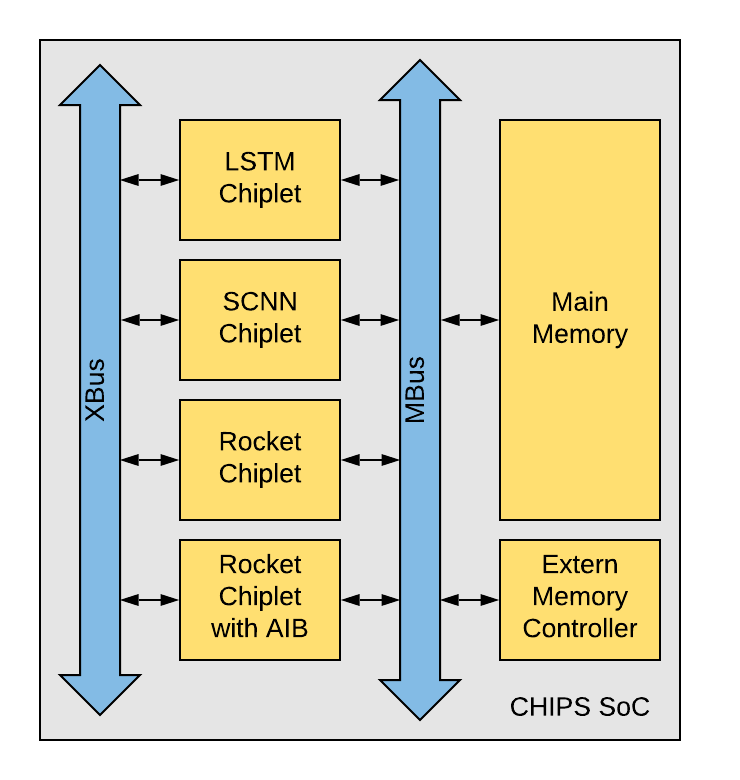
\includegraphics[scale=.27]{pngs/CHIPS-system.png}
    \caption{CHIPS SOC}
    \label{fig:CHIPS-arch}
\end{figure}

The CHIPS SoC consists of two bus types debug (JTag) and memory (AXI). JTag allows interaction control over the chiplets and the SoC sub-system. The SoC contains two AXI bus: one is for on and off-chip memory access (MBus), and the other is for neural network chiplet control (XBus).  The MBus allows each chiplet to connect to the on-chip memory. The external memory controller bridges the MBus with the off-chip memory using the CIPI protocol. The XBus allows the Rocker chiplets to control the behavior of the neural network chiplets. Figure \ref{fig:CHIPS-arch} shows an overview of the Chips SoC. 


\subsection{Chiplets}
As stated in the section before, each chiplet has three bus connections. For controller chiplets, Rocket cores, they have two master AXI ports, XBus and MBus, and one JTag debug port. For the neural network chiplets, they have one master AXI port, MBus, one slave port AXI port, XBus, and one Jtag debug port.

\subsubsection{Rocket Chiplet}
The Rocket chiplet had to be modified to work in the CHIPS architecture. In this version of the Rocket chiplet, there is no floating-point hardware, and there is support for the E instructions extensions. Only one of the E instruction extensions is used to control access to the XBus. This instruction has two variants, bus read and bus write. These two actions allow the Rocket core to control and debug the neural network chiplets via XBus

\subsubsection{Neural Network Chiplets}
In this architecture, there are two neural network chiplets: LSTM and SCNN. Both chiplets are accessible via JTag port or XBus port. These chiplets are designed to work at the coarse grain programming level. 

The LSTM chiplet is the product of Dr. Summon Dey's dissertation research at NCSU. The following is an overview of his chiplet design\cite{Summon-Dey-LSTM}. The LSTM chiplet focuses on developing hardware that can fully utilize its memory bandwidth. So, his chiplet scales with the amount of memory bandwidth available. In addition to scaling with the memory bandwidth, it needs to be able to adaptable to changes in recurrent neural networks (RNN) algorithms. To this end, he based his design on a very long instruction word (VLIW) architecture. In this style of architecture, a single instruction represents a set to micro-opts. Each micro-opt controls a section/lane of the design. See his paper for more details on his design\cite{Summon-Dey-LSTM}.

The SCNN chiplet is the product of Dr. Weifu Li's dissertation research at NCSU. The following is an overview of his chiplet design\cite{LeWeifuDissertation}. His chiplet design focus on reducing the amount of memory access need to process a CNN. To this end, he uses a run-length encoding (RLE) format to compress the zeros in the input feature data and weights. His hardware uses the RLE data to reduce the amount of memory access to memory.

\end{document}

